\section{Análisis de la obra pictórica: Cristo crucificado de el Greco}

\begin{figure}[ht!]
    \centering
    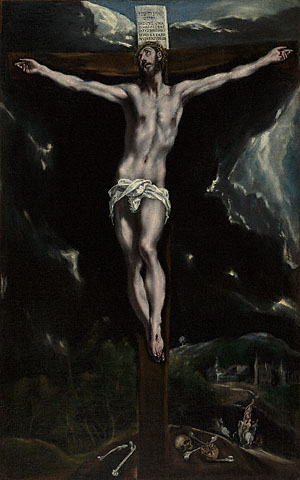
\includegraphics[width=0.9\textwidth]{elgreco.jpg}
   .\caption{Cristo crucificado de El Greco. Museo J. Paul Getty.} % URL: www.getty.edu/art/gettyguide/artObjectDetails?artobj=138292\&handle=li}
\end{figure}

\newpage

%Arte, estilo: Manierismo
%Cronología: Hacia 1600-1610
%Lugar: Museo J. Paul Getty, Los Ángeles
%Autor: El Greco
%Título: Cristo crucificado 

%Función: Purchased by a Spanish family at a flea market around 1950, it remained in their possession until recently. 
% http://www.ctv.es/USERS/ags/00013_mm.htm
% http://www.google.com/culturalinstitute/asset-viewer/christ-on-the-cross/cgHO8uo2dVOJoQ?hl=es&projectId=art-project


\begin{description}
\item[Estilo] Manierismo
\item[Cronología] Hacia 1600-1610
\item[Lugar] Museo J. Paul Getty, Los Ángeles
\item[Autor] Doménikos Theotokópoulos, más conocido como el Greco
\item[Título] Cristo crucificado
\end{description}

\textbf{Contexto histórico:}

El cuadro se realizó en plena contrarreforma. Durante este período la Iglesia católica intentaba consolidar su poder bajo la amenaza de la reforma protestante, es por eso que durante esta época se produjeron un gran número de obras de contenido religioso. De hecho la gran mayoría de las obras elaboradas por el Greco son de naturaleza religiosa, centrándose menos en retratos u otro estilo de obras. La obra a analizar es una de estas obras de carácter religioso.

En esta, y en general en todas sus obras, el Greco utilizaba un estilo propio basándose en el estilo veneciano en el uso del color y en el Manierismo alargando y retorciendo las formas y figuras. Dejó, de esta forma a un lado el orden, la claridad, la proporción y el equilibrio característico del Renacimiento anterior.

Se observan grandes contrastes en el uso del color en esta obra. Las figuras parecen emanar luz propia, pues están envueltas en oscuridad y exclusivamente hay luz en las formas que el autor quería que advirtiésemos. Además, esta utilización del color nos lleva a discernir la sombría situación del calvario de Cristo.

El alargamiento de las formas, propio de el Greco, provee a la obra de mayor belleza y misticismo, lo que le valió el reconocimiento de muchos religiosos de la época.

Siguiendo el estilo de su época el Greco representó la crucifixión de Cristo mediante tres clavos: un clavo que junta ambos pies a la cruz directamente y un clavo en cada palma de la mano, según la interpretación bíblica de la época, contrariamente a la creencia actual principal de que se encontraban a la altura de las muñecas.


\vspace{12pt}
\textbf{Anatomía de superficie:}

En esta obra el Greco nos muestra un Cristo que presenta una anatomía adecuada excepto en sus proporciones. La figura sigue una proporción de nueve cabezas, pudiendo apreciar, efectivamente la cabeza pequeña de la figura mientras el tronco y sus extremidades son extremadamente alargados, no concordando con ningún cánon de proporciones habitual \footnote{Actualmente existen tres cánones para determinar las proporciones de la figura humana: el cánon de siete cabezas y media, el cánon más relista en cuanto a medidas, que se considera la figura común, el cánon de ocho cabezas considerado la figura ideal y el cánon de ocho cabezas y media, con el que se representan las figuras heróicas.}. Sin embargo estas medidas dotan a la figura de una mayor heroicidad, presentando de esta forma, y junto con otros detalles de la obra, el triunfo de Cristo sobre la muerte, idea que en la contrarreforma querían destacar. Su longitud con los brazos extendidos es igual a su altura y el ángulo que forman entre ellos es de 135º.

Como la figura no ha fallecido no es posible observar las características típicas de la muerte como es la lividez del cuerpo o la laxitud muscular. Es más, la figura conserva los ojos abiertos, mostrando una ausencia de sufrimiento en el rostro, lo que es otro detalle de la obra en la que se ilustra el triunfo de Cristo, que inexpresivo mira al cielo (a Dios) a la espera de su muerte. La posición retorcida del cuerpo es utilizada por el autor para aumentar la belleza del cuadro, sin reparar en que es extremadamente difícil adquirir esa posición estando crucificado y al borde de la muerte. Tanto los músculos de los brazos como los de las piernas que contribuyen al mantenimiento de la postura están contraídos y extendidos, sin embargo los de la espalda, muy necesarios para el mantenimiento de esta postura no se observan claramente.

Apoya la mayor parte del peso del cuerpo sobre la pierna derecha aprovechando para inclinar la cadera hacia el mismo lado produciendo la curvatura del cuerpo de la que he hablado anteriormente y que se continuará en forma de \textit{S} a lo largo de la figura.

Además, existen otros signos que muestran el triunfo de la vida sobre la muerte. Uno de ellos es la escasa sangre que se visualiza en este cuadro, quitando de esta manera importancia a las heridas de la carne y dando una apariencia más divina. No encontramos la herida del costado derecho, lo que, de hecho, es lógico debido a que esta se le ocasiona después de morir, para verificar su muerte.

Para conseguir la postura que mantiene la figura intervienen varios músculos.
Tanto la espalda como el cuello se encuentran en posición erguida, con el rostro mirando hacia arriba, utilizando para ello los músculos erectores de la columna: los músculos del grupo iliocostal, los del grupo longuísimo y los del espinoso y los principales músculos del cuello como el esplenio y el esternocleidomastoideo, este último visible en la obra. Otro músculo que participa en la postura erecta es el recto del abdomen, el cual se puede discernir en la obra, junto con la línea alba, formada por la unión de vainas fibrosas en la línea media, y la línea semilunar, que marca el borde lateral del músculo recto del abdomen.

El músculo dorsal ancho que proviene de la espalda posee un tendón estrecho que envuelve al músculo redondo mayor formando el pliegue posterior de la axila, reconocible en esta imagen. Estos músculos producen la elevación del tronco estando los brazos fijos, por tanto tienen gran relevancia en la crucifixión. Además de estos dos músculos otro que participa en la elevación del tronco es el pectoral mayor que forma el pliegue anterior de la axila, también visible en la obra.

Otros músculos con gran relevancia en esta posición son: el trapecio, que se puede observar en la figura, y el elevador de la escápula, que elevan la escápula, y el serrato anterior que la gira. La posicion de Cristo en la cruz desplaza la escápula de esta forma.

El músculo deltoides se aprecia sin esfuerzo rodeando la articulación de los hombros en ambas extremidades superiores. Su principal función es la abducción del brazo y es por eso que se le confiere gran importancia en la posición en la que ambos brazos están en abducción.

En el brazo, aunque no con trazos muy firmes, son evidentes los músculos bíceps y tríceps. El primero se encuentra en la parte anterior del brazo y su principal función es la flexión de la articulación del codo, sin embargo en esta figura los brazos se encuentran en extensión por la que la función principal del bíceps no es la anteriormente citada sino la supinación del antebrazo, la cual la realiza junto con el músculo supinador. Por su parte el tríceps se encuentra en la parte posterior siendo su principal función la extensión de la articulación del codo, lo que posee importancia en esta posición. 

Las manos se encuentran en posición de reposo, por lo que el tercer, cuarto y quinto dedo se encuentran ligeramente flexionados, no siendo así, sin embargo, en el primer y el segundo dedo que se encuentran extendidos, posiblemente debidos a los clavos con los que se sujeta a la figura en la cruz. Estos no están representados en el centro de las palmas de las manos, como era habitual, si no que se sitúan entre los segundos y terceros huesos metacarpianos.

La caja torácica es fácilmente visible: el borde costal inferior, la depresión en la que se encuentra el esternón, algunas costillas (probablemente la tercera y la cuarta) e, incluso, ambas clavículas elevadas debido a la elevación de los brazos, que a su vez hace posible la óptima visualización de las estructuras anteriormente citadas. Igualmente, como el autor de la obra representa a un Cristo más bien delgado, la espina ilíaca puede ser divisada superficialmente en ambos lados de la pelvis.

La extremidad inferior izquierda mantiene la articulación de la rodilla ligeramente flexionada, mientras que la derecha la mantiene totalmente extendida. A su vez la cadera se encuentra ladeada hacia el lado de la pierna estirada, provocando que la espina ilíaca sea más fácilmente visible en este costado que en el izquierdo.
Los encargados de mantener esta postura son: en la extensión, el cuadriceps y los músculos del tracto iliotibial, y en la flexión, los músculos poplíteos y los gemelos. La rótula o patella, que se encuentra en la articulación de la rodilla se vislumbra perfectamente junto con la tuberosidad tibial en la rodilla flexionada. Aún así, la tuberosidad tibial, anatómicamente recta desde la articulación de la rodilla hasta la articulación del tobillo, se presenta curvada en el afán de el Greco por moldear las formas a su antojo

Los pies se encuentran uno sobre otro,el izquierdo sobre el derecho, y ambos clavados juntos en la cruz. Mantienen el peso de la mayor parte del cuerpo, ayudados por los músculos que elevan el tronco y los clavos que sujetan ambos brazos.